\documentclass[tikz,border=8pt]{standalone}
\usepackage{amsmath}
\usepackage{amssymb}
\usepackage{tikz}
\usetikzlibrary{arrows.meta,calc,decorations.pathreplacing,patterns,shapes.geometric,positioning,shadings,plotmarks}

\begin{document}
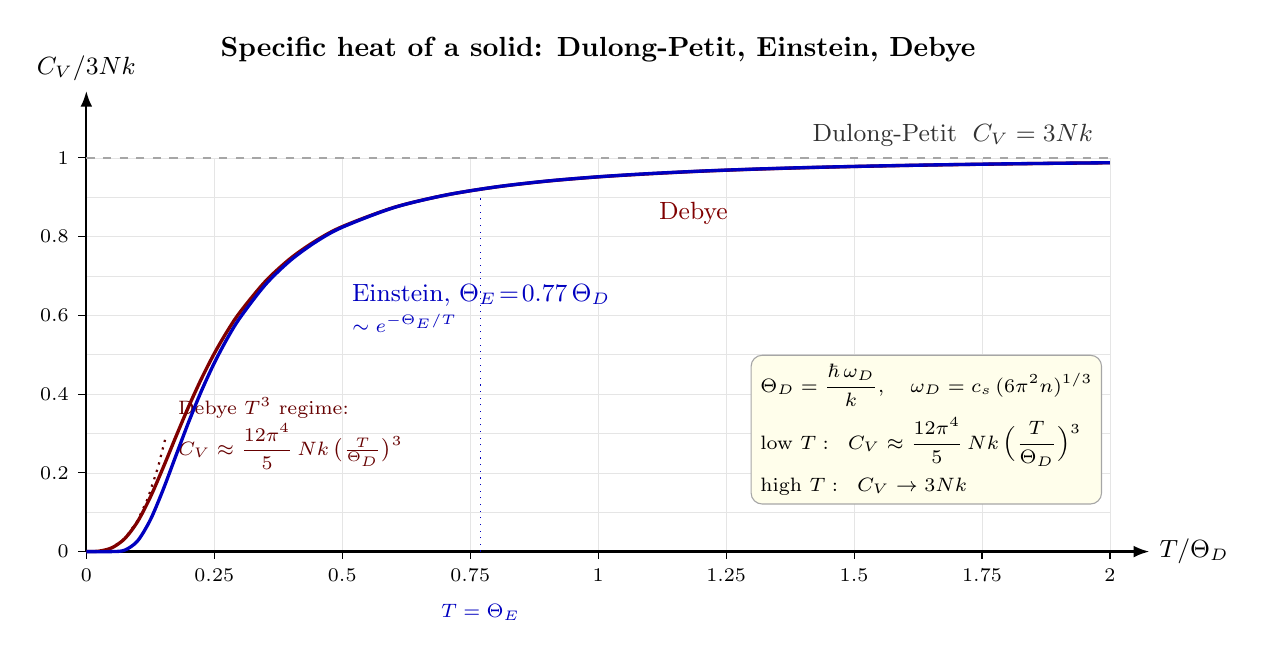
\begin{tikzpicture}[
    >={Latex[length=2mm]},
    font=\small
]

% =============================================
% C_V / (3Nk) vs T/Theta_D
% Three curves:
%   Dulong-Petit: horizontal at 1
%   Einstein:      Theta_E = 0.77 Theta_D, exponential freeze-out
%   Debye:         numerical Debye integral, T^3 onset
% =============================================

\def\xscale{6.5}    % cm per (T/Theta_D)
\def\yscale{5.0}    % cm per unit (C_V / 3Nk)
\def\xmax{2.0}
\def\ymax{1.05}

% Light grid
\draw[very thin, gray!20]
   (0,0) grid[xstep=0.25*\xscale, ystep=0.1*\yscale]
   (\xmax*\xscale, 1.0*\yscale);

% Axes
\draw[->, thick] (0,0) -- (\xmax*\xscale+0.5,0)
   node[right] {$T/\Theta_D$};
\draw[->, thick] (0,0) -- (0,\ymax*\yscale+0.6)
   node[above] {$C_V / 3Nk$};

% X tick labels
\foreach \x/\lab in {0/0, 0.25/0.25, 0.5/0.5, 0.75/0.75, 1/1, 1.25/1.25, 1.5/1.5, 1.75/1.75, 2/2}{
   \draw (\x*\xscale,0) -- (\x*\xscale,-0.1) node[below] {\scriptsize $\lab$};
}
% Y tick labels
\foreach \y/\lab in {0/0, 0.2/0.2, 0.4/0.4, 0.6/0.6, 0.8/0.8, 1/1}{
   \draw (0,\y*\yscale) -- (-0.1,\y*\yscale) node[left] {\scriptsize $\lab$};
}

% --- Dulong-Petit horizontal line at C_V/(3Nk) = 1 ---
\draw[dashed, thick, gray!70]
   (0, 1*\yscale) -- (\xmax*\xscale, 1*\yscale);
\node[gray!40!black, anchor=south west, font=\small]
   at (1.40*\xscale, 1.005*\yscale) {Dulong-Petit $\;C_V = 3Nk$};

% --- Debye low-T cubic asymptote (dotted) ---
% In units of 3Nk:  C_V/(3Nk) = (4 pi^4 / 5) (T/Theta_D)^3 = 77.93 t^3.
\draw[dotted, thick, red!40!black]
   plot coordinates {
     (0,0)
     ({0.025*\xscale}, {77.93*0.025*0.025*0.025*\yscale})
     ({0.050*\xscale}, {77.93*0.050*0.050*0.050*\yscale})
     ({0.075*\xscale}, {77.93*0.075*0.075*0.075*\yscale})
     ({0.100*\xscale}, {77.93*0.100*0.100*0.100*\yscale})
     ({0.120*\xscale}, {77.93*0.120*0.120*0.120*\yscale})
     ({0.140*\xscale}, {77.93*0.140*0.140*0.140*\yscale})
     ({0.155*\xscale}, {77.93*0.155*0.155*0.155*\yscale})
   };

% --- Annotation arrow for the Debye T^3 region ---
\node[red!40!black, anchor=west, font=\scriptsize, align=left]
   at (0.16*\xscale, 0.30*\yscale)
   {Debye $T^{3}$ regime: \\[1pt]
    $C_V \approx \dfrac{12\pi^{4}}{5}\,Nk\,\bigl(\tfrac{T}{\Theta_D}\bigr)^{3}$};

% =============================================
% Debye exact curve (numerical integration of Debye formula)
% Coordinates: (T/Theta_D, C_V/(3Nk))
% =============================================
\draw[very thick, red!50!black, smooth]
   plot coordinates {
     (0,0)
     ({0.025*\xscale}, {0.0012*\yscale})
     ({0.050*\xscale}, {0.0097*\yscale})
     ({0.075*\xscale}, {0.0328*\yscale})
     ({0.100*\xscale}, {0.0758*\yscale})
     ({0.125*\xscale}, {0.1382*\yscale})
     ({0.150*\xscale}, {0.2130*\yscale})
     ({0.175*\xscale}, {0.2919*\yscale})
     ({0.200*\xscale}, {0.3686*\yscale})
     ({0.225*\xscale}, {0.4395*\yscale})
     ({0.250*\xscale}, {0.5031*\yscale})
     ({0.275*\xscale}, {0.5590*\yscale})
     ({0.300*\xscale}, {0.6077*\yscale})
     ({0.350*\xscale}, {0.6866*\yscale})
     ({0.400*\xscale}, {0.7459*\yscale})
     ({0.450*\xscale}, {0.7908*\yscale})
     ({0.500*\xscale}, {0.8254*\yscale})
     ({0.600*\xscale}, {0.8738*\yscale})
     ({0.700*\xscale}, {0.9050*\yscale})
     ({0.800*\xscale}, {0.9260*\yscale})
     ({0.900*\xscale}, {0.9409*\yscale})
     ({1.000*\xscale}, {0.9517*\yscale})
     ({1.100*\xscale}, {0.9596*\yscale})
     ({1.200*\xscale}, {0.9661*\yscale})
     ({1.300*\xscale}, {0.9710*\yscale})
     ({1.400*\xscale}, {0.9749*\yscale})
     ({1.500*\xscale}, {0.9781*\yscale})
     ({1.600*\xscale}, {0.9807*\yscale})
     ({1.700*\xscale}, {0.9829*\yscale})
     ({1.800*\xscale}, {0.9847*\yscale})
     ({1.900*\xscale}, {0.9863*\yscale})
     ({2.000*\xscale}, {0.9876*\yscale})
   };

\node[red!50!black, anchor=west, font=\small]
   at (1.10*\xscale, 0.86*\yscale) {Debye};

% =============================================
% Einstein curve, Theta_E = 0.77 Theta_D
% Coordinates: (T/Theta_D, C_V/(3Nk))
% =============================================
\draw[very thick, blue!75!black, smooth]
   plot coordinates {
     (0,0)
     ({0.050*\xscale}, {0.0000*\yscale})
     ({0.075*\xscale}, {0.0037*\yscale})
     ({0.100*\xscale}, {0.0269*\yscale})
     ({0.125*\xscale}, {0.0805*\yscale})
     ({0.150*\xscale}, {0.1572*\yscale})
     ({0.175*\xscale}, {0.2436*\yscale})
     ({0.200*\xscale}, {0.3293*\yscale})
     ({0.225*\xscale}, {0.4085*\yscale})
     ({0.250*\xscale}, {0.4790*\yscale})
     ({0.275*\xscale}, {0.5405*\yscale})
     ({0.300*\xscale}, {0.5935*\yscale})
     ({0.350*\xscale}, {0.6783*\yscale})
     ({0.400*\xscale}, {0.7410*\yscale})
     ({0.450*\xscale}, {0.7880*\yscale})
     ({0.500*\xscale}, {0.8238*\yscale})
     ({0.600*\xscale}, {0.8734*\yscale})
     ({0.700*\xscale}, {0.9050*\yscale})
     ({0.800*\xscale}, {0.9262*\yscale})
     ({0.900*\xscale}, {0.9412*\yscale})
     ({1.000*\xscale}, {0.9520*\yscale})
     ({1.100*\xscale}, {0.9601*\yscale})
     ({1.200*\xscale}, {0.9664*\yscale})
     ({1.300*\xscale}, {0.9713*\yscale})
     ({1.400*\xscale}, {0.9752*\yscale})
     ({1.500*\xscale}, {0.9783*\yscale})
     ({1.600*\xscale}, {0.9809*\yscale})
     ({1.700*\xscale}, {0.9831*\yscale})
     ({1.800*\xscale}, {0.9849*\yscale})
     ({1.900*\xscale}, {0.9864*\yscale})
     ({2.000*\xscale}, {0.9877*\yscale})
   };

\node[blue!75!black, anchor=west, font=\small]
   at (0.50*\xscale, 0.65*\yscale)
   {Einstein, $\Theta_E\!=\!0.77\,\Theta_D$};
\node[blue!75!black, anchor=west, font=\scriptsize]
   at (0.50*\xscale, 0.58*\yscale) {$\sim e^{-\Theta_E/T}$};

% Thin pointer line for Theta_E
\draw[blue!75!black, dotted]
   (0.77*\xscale, 0) -- (0.77*\xscale, 0.91*\yscale);
\node[blue!75!black, font=\scriptsize, anchor=north]
   at (0.77*\xscale, -0.55) {$T = \Theta_E$};

% =============================================
% Boxed reference equations
% =============================================
\node[draw=gray!70, fill=yellow!8, rounded corners,
      align=left, font=\scriptsize, anchor=north east]
   at (\xmax*\xscale-0.1, 0.50*\yscale)
   {$\Theta_D = \dfrac{\hbar\,\omega_D}{k},\quad
     \omega_D = c_s\,(6\pi^{2} n)^{1/3}$ \\[3pt]
     low $T:\;\;
       C_V \approx \dfrac{12\pi^{4}}{5}\,Nk\,\Bigl(\dfrac{T}{\Theta_D}\Bigr)^{3}$ \\[3pt]
     high $T:\;\;C_V \to 3Nk$};

% Title
\node[above, font=\bfseries] at (\xmax*\xscale/2, \ymax*\yscale+0.85)
   {Specific heat of a solid: Dulong-Petit, Einstein, Debye};

\end{tikzpicture}
\end{document}
